\documentclass{beamer}
\usepackage{amsmath,amssymb,amsthm,tikz,color,wrapfig}
\usetheme{metropolis}
\setbeamertemplate{footline}[default]

\definecolor{azure}{rgb}{0.4, 0.2, 1.0}
\definecolor{cinnamon}{rgb}{0.82, 0.41, 0.12}
\definecolor{bur}{rgb}{0.6, 0.0, 0.0}

\title{Computing Galois groups of Fano problems}
\author{Thomas Yahl\\  \texttt{thomasjyahl@tamu.edu}\\ \vspace{-.1cm} \\ \texttt{arXiv:}\\ \vspace{-.1cm} \\ Texas A\&M University}
\date{June 2022}




%%%%%%%%%%%%
%%Commands%%
%%%%%%%%%%%%
\newcommand{\new}[1]{{\color{black!10!blue}#1}}
\newcommand{\blue}[1]{{\color{black!10!blue}\underline{#1}}}
\newcommand{\orange}[1]{{\color{black!15!cinnamon}\underline{#1}}}


%%%%%%%%%%%%%%%%%
%%Rough Outline%%
%%%%%%%%%%%%%%%%%
%Computing Galois groups of Fano problems
%
%1. 27 lines (1 slide + picture)
%      mention "remakable configuration of lines"
%      Fano problems are generalizations of this
%   
%2. Fano problems (1 slide w/ example)
%      definition
%      dimension/degree (DM)
%      finite Fano problems
%      (1,6,(2,2,3)) example
%   
%3. Galois groups (2 slide + picture/gif?)
%      incidence variety
%      Galois group is monodromy group
%      path lifting (w/ picture)
%   
%4. Known results (1 slide)
%      Jordan/Harris for 27 lines
%      Hoshimoto & Kadets
%      remaining problems are alternating or symmetric
%      explore and prove with numerics
%
%5. Monodromy via homotopy continuation (3 slides, "would like to turn into proof")
%      necessary homotopy continuation slide (w/ picture)
%      small discriminant loop output for 27 lines and (1,6,(2,2,3))
%      computations, this is evidence we want proof
%
%6. Harris' method (1 slide + picture)
%      (1,n,(2n-3)) have symmetric Galois groups
%      Harris' method of proof (w/ picture)
%      this can be done computationally
%
%7. Certification (maybe 3 slides? picture? emphasize hard certification)
%      Smale's alpha theory
%      interval arithmetic
%      Shub's simple double roots
%
%8. Computations
%      constructing systems with unique simple double roots
%      certifying them w/ alpha theory/interval arithmetic + Shub
%      timings
%
%9. Moving forward
%      more computations
%      proving the result for all Fano problems
%

\begin{document}

%title frame
\begin{frame}
\titlepage

\texttt{arXiv:}
\end{frame}


%Frame 2
%27 lines (1 slide + picture)
%%mention "remakable configuration of lines"
%%Fano problems are generalizations of this
\begin{frame}
\frametitle{The problem of lines on a cubic surface}
\hspace{-.8cm}
\begin{minipage}{.55\textwidth}
\begin{enumerate}
\item[$\bullet$] Cayley and Salmon showed there are 27 distinct lines that lie on a smooth cubic surface.

\item[$\bullet$] Schl\"{a}fli determined these lines lie in a ``remarkable configuration'' 

\item[$\bullet$] This is an instance of a \blue{Fano problem}.
\end{enumerate}
\end{minipage}
%
\begin{minipage}{.02\textwidth}
~
\end{minipage}
%
\begin{minipage}{.4\textwidth}
%27 lines picture
\begin{center}
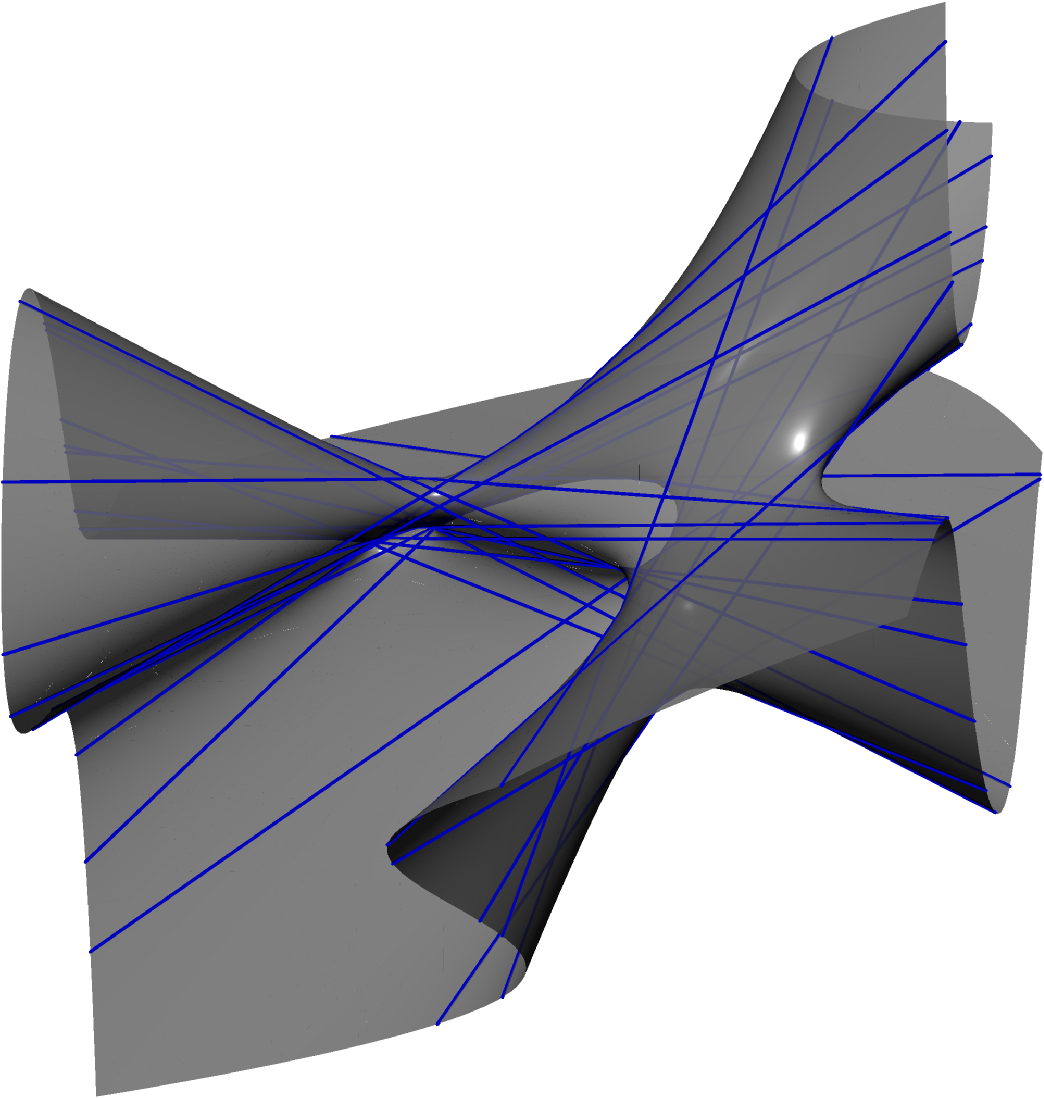
\includegraphics[scale=.32]{figures/27lines.pdf}
\end{center}
\end{minipage}


\end{frame}


%Frame 3
%Fano problems (1 slide w/ example)
%%definition
%%dimension/degree (DM)
%%finite Fano problems
%%(1,6,(2,2,3)) example
\begin{frame}
\frametitle{Fano problems}
\begin{enumerate}
\item[$\bullet$] For fixed degrees $d_\bullet = (d_1,\dotsc,d_s)$ choose homogeneous polynomials in $n+1$ variables, $F = (f_1,\dotsc,f_s)$.

\item[$\bullet$] Enumerate the $r$-planes that lie on the zero set $X = V(F)\subseteq\mathbb{P}^n$.
\end{enumerate}

When there are finitely many such $r$-planes for general polynomials $F = (f_1,\dotsc,f_s)$, this is a \blue{Fano problem} determined by $(r,n,d_\bullet)$.

\begin{enumerate}
\pause

\item[$\bullet$] The set of $r$-planes on $X=V(F)$, written $V_r(F)$, is a subvariety of the Grassmanian $\mathbb{G}(r,\mathbb{P}^n)$.

\pause

\item[$\bullet$] The combinatorial data $(r,n,d_\bullet)$ determines a Fano problem when $n-s-2r\ge 0$ and

\vspace{-.8cm}

\begin{align*}
(r+1)(n-r) = \sum_{i=1}^s \left(\begin{smallmatrix}d_i + r\\r\end{smallmatrix}\right).
\end{align*}
\end{enumerate}

\end{frame}

%Frame 4
%rewrite this slide
\begin{frame}
\frametitle{Examples}
Debarre and Manivel determined the number of solutions to the Fano problem determined by the data $(r,n,d_\bullet)$ by intersection theoretic means.

By exhaustion, we enumerate Fano problems of small size.

\begin{table}[htb]
  \label{Small Fano}
  \def\arraystretch{1.1}
  \begin{tabular}{||c|c|c|c|c||}
    \hline
    $r$ & $n$ & $d_\bullet$ & $\#$ of solutions & Galois group\\
    \hline\hline
    1 & 4 & $(2,2)$ & 16 & $D_5$\\
    \hline
    1 & 3 & $(3)$ & 27 & $E_6$\\
    \hline
    2 & 6 & $(2,2)$ & 64 & $D_7$\\
    \hline
    3 & 8 & $(2,2)$ & 256 & $D_9$\\
    \hline
    1 & 7 & $(2,2,2,2)$ & 512 & \new{$S_{512}$}\\
    \hline
    1 & 6 & $(2,2,3)$ & 720  & \new{$S_{720}$}\\
    \hline
  \end{tabular}
\end{table}
\end{frame}


%Frame 5
%Galois groups (2 slide + picture/gif?)
%%incidence variety
%%Galois group is monodromy group
%%path lifting (w/ picture)
\begin{frame}
\frametitle{Incidence correspondence}
Write $\mathbb{C}^{(r,n,d_\bullet)}$ for the parameter space of homogeneous forms $(f_1,\dotsc,f_s)$ in $n+1$ variables of degrees $d_\bullet = (d_1,\dotsc,d_s)$.

%For the Fano problem determined by $(r,n,d_\bullet)$, there is an incidence correspondence
Fix $(r,n,d_\bullet)$. There is an incidence correspondence

\vspace{-.3cm}

\begin{center}
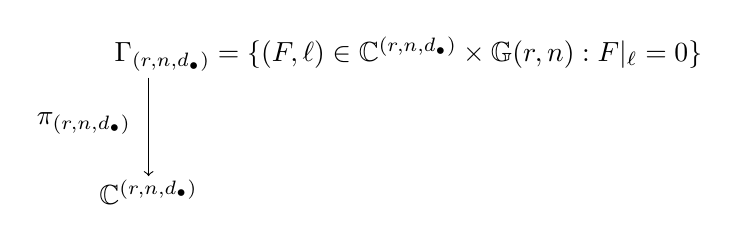
\begin{tikzpicture}
\node at (0,0) {$\Gamma_{(r,n,d_\bullet)} = \{(F,\ell)\in \mathbb{C}^{(r,n,d_\bullet)}\times\mathbb{G}(r,n):F|_\ell = 0\}$};
\node at (-3.3,-1.75) {$\mathbb{C}^{(r,n,d_\bullet)}$};
\draw[->] (-3.3,-.3)--(-3.3,-1.55) node[left] at (-3.4,-.875) {$\pi_{(r,n,d_\bullet)}$};
\end{tikzpicture}
\end{center}

\vspace{-.45cm}

\begin{enumerate}
\item[$\bullet$] $\Gamma_{(r,n,d_\bullet)}$ is irreducible.

\item[$\bullet$] The fiber over $F\in\mathbb{C}^{(r,n,d_\bullet)}$ is the set of $r$-planes $V_r(F)$.

\item[$\bullet$] $\pi$ restricts to a covering space over a Zariski open set $U_{(r,n,d_\bullet)}\subseteq\mathbb{C}^{(r,n,d_\bullet)}$.

\end{enumerate}
\end{frame}


%Frame 6
\begin{frame}
\frametitle{Galois groups of Fano problems}
\hspace{-.65cm}
\begin{minipage}{.73\textwidth}
\begin{enumerate}
\item[$\bullet$] The \blue{Galois group}, $\mathcal{G}_{(r,n,d_\bullet)}$, of the Fano problem determined by $(r,n,d_\bullet)$ is the monodromy group of $\pi_{(r,n,d_\bullet)}$.

\vspace{.1cm}

\item[$\bullet$] Jordan showed $\mathcal{G}_{(1,3,(3))}\subseteq E_6$.

\vspace{.1cm}

\item[$\bullet$] Harris showed $\mathcal{G}_{(1,3,(3))} = E_6$ and $\mathcal{G}_{(1,n,(2n-3))}$ is symmetric.

\vspace{.1cm}

\item[$\bullet$] Hashimoto and Kadets showed $\mathcal{G}_{(r,2r+2,(2,2))}=D_{2r+3}$ and $\mathcal{G}_{(r,n,d_\bullet)}$ \\
contains the alternating group for \\
remaining Fano problems.
\end{enumerate}
\end{minipage}
%
\begin{minipage}{.25\textwidth}
\begin{center}
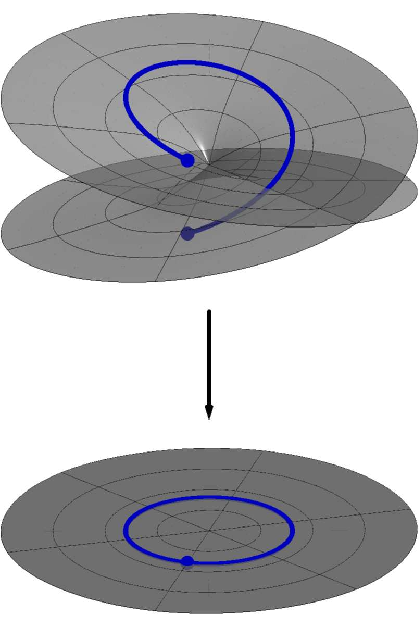
\includegraphics[scale=.5]{figures/monodromy.pdf}
\end{center}
\end{minipage}

\vspace{.15cm}

\textbf{\underline{Goal:}} use numerics \underline{prove} remaining Galois groups are symmetric. 

\end{frame}

%Frame 7
%Monodromy via homotopy continuation (2 slides, "would like to turn into proof")
%%necessary homotopy continuation slide (w/ picture)
%%small discriminant loop output for 27 lines and (1,6,(2,2,3))
%%computations, this is evidence we want proof
%\begin{frame}
%\frametitle{Numerical homotopy continuation}


%Numerical homotopy picture
%\begin{center}
%\begin{tikzpicture}
%\draw[thick,<->] (-2.75,0)--(2.75,0) node [right] at (2.75,0) {$t$};
%\draw[dashed] (-2,-.75)--(-2,1.75) node [below] at (-2,-.75) {$\mathcal{F}$};
%\draw[dashed] (2,-.75)--(2,1.75) node [below] at (2,-.75) {$\mathcal{G}$};

%\draw[blue,fill=blue] (2,-.3) circle (.05cm);
%\draw[blue,fill=blue] (-2,.3) circle (.05cm);
%\draw[blue,thick] (2,-.3)..controls(.9,-.5)..(.2,.6)..controls(-.1,1)..(-.65,.8);
%\draw[blue,thick] (-.85,.7)..controls(-1,.65)..(-2,.3);

%\draw[black!30!green,fill=black!30!green] (2,.15) circle (.05cm);
%\draw[black!30!green,fill=black!30!green] (-2,1.5) circle (.05cm);
%\draw[black!30!green,thick] (2,.15)..controls(1.5,.3)..(.8,-.1);
%\draw[black!30!green,thick] (.6,-.2)..controls(.3,-.3)..(-.3,.35)..controls(-1,1)..(-2,1.5);

%\draw[black!15!red,fill=black!15!red] (2,1.4) circle (.05cm);
%\draw[black!15!red,thick] (2,1.4)..controls(1.2,1)..(.4,1.2)..controls(-.5,1.4)..(-1,1.1);
%\draw[black!15!red,thick] (-1.2,.9)..controls(-1.3,.8)..(-1.45,.6);
%\draw[black!15!red,thick,->] (-1.6,.35)..controls(-1.75,.1)..(-1.85,-.6);
%\end{tikzpicture}
%\end{center}


%\end{frame}

%Frame 8
%\begin{frame}
%\frametitle{Computations}

%\end{frame}


%Frame 9
%Harris' method (1 slide + picture)
%%(1,n,(2n-3)) have symmetric Galois groups
%%Harris' method of proof (w/ picture)
%%this can be done computationally
\begin{frame}
\frametitle{Harris' method of proof}

To show $\mathcal{G}_{(1,n,(2n-3))}$ is contains a simple transposition, Harris showed the existence of $p\in U_{(1,n,(2n-3))}$ satisfying the following.

\begin{lemma}[Harris]

\vspace{.05cm}

Let $\pi:Y\mapsto X$ be a smooth map of degree $n$ between irreducible varieties. If there exists a point $p\in X$ such that the fiber $\pi^{-1}(p)$ consists of exactly $n-2$ simple points and one double point then the monodromy group of $\pi$ contains a simple transposition.
\end{lemma}

\begin{enumerate}
\pause

\item[$\bullet$] For remaining Fano problems of moderate size, we construct $p\in U_{(r,n,d_\bullet)}$ satisfying the above.

\pause

\item[$\bullet$] To prove the constructed systems satisfy the above, we make use of numerical certification.

\end{enumerate}
\end{frame}


%Frame 10
%Certification (maybe 2 slides? picture? emphasize hard certification)
%%Smale's alpha theory
%%interval arithmetic
%%Shub's simple double roots
\begin{frame}
\frametitle{Numerical certification}
\begin{enumerate}
\item[$\bullet$] Smale's $\alpha$-theory

\item[$\bullet$] Interval arithmetic

\end{enumerate}
\end{frame}

%Frame 11
\begin{frame}
\frametitle{Example}

\end{frame}


%Frame 12
%Computations
%%constructing systems with unique simple double roots
%%certifying them w/ alpha theory/interval arithmetic + Shub
%%timings
\begin{frame}
\frametitle{Constructing systems with a unique simple double root}

\end{frame}

%Frame 13
\begin{frame}
\frametitle{Results and timings}

\end{frame}


%Frame 14
%Moving forward
%more computations
%proving the result for all Fano problems
\begin{frame}
\frametitle{Moving forward}

\end{frame}

%Frame 15
\begin{frame}
\frametitle{References}

\end{frame}

\end{document}





\begin{table}[htb]
  \label{Small Fano}
  \def\arraystretch{1.1}
  \begin{tabular}{||c|c|c|c||}
    \hline
    $r$ & $n$ & $d_\bullet$ & $\#$ of solutions\\
    \hline\hline
    1 & 4 & $(2,2)$ & 16\\
    \hline
    1 & 3 & $(3)$ & 27 \\
    \hline
    2 & 6 & $(2,2)$ & 64 \\
    \hline
    3 & 8 & $(2,2)$ & 256 \\
    \hline
    1 & 7 & $(2,2,2,2)$ & 512 \\
    \hline
    1 & 6 & $(2,2,3)$ & 720 \\
    \hline
  \end{tabular}
\end{table}


